

\subsubsection*{Netzwerk-Applikationen und Protokolle}

\begin{KR}{Übersicht Applikationsprotokolle}
    \begin{itemize}
        \item Das Domain Name System (DNS) erlaubt übersetzt Hostnamen in IP Adressen und umgekehrt
        \begin{itemize}
            \item Besteht aus einem hierarchischen DNS Name Space
            \item Das DNS wird auf einer grossen Anzahl Name Server verteilt betrieben, ein Name Server ist jeweils für eine Zone verantwortlich (z.B. zhaw.ch)
        \end{itemize}
        \item DHCP erlaubt einem Rechner, seine IP Konfiguration von einem Server zu beziehen
        \item TFTP ist ein einfaches, aber zuverlässiges File Transfer Protocol, welches z.B. diskless Systemen dazu dient, das Betriebssystem Image vom Server zu beziehen
        \item HTTP erlaubt den Zugriff auf verteilte Dokumente, die mittels Uniform Resource Locator (URL) eindeutig adressiert werden
        \item Network Address Translation (NAT) erlaubt die Wiederverwendung privater IP-Adressen
    \end{itemize}
\end{KR}

\section{Application Layer}

\paragraph{DNS - Domain Name Space}

\begin{definition}{DNS} Name Resolution (IP Adr. leserlich machen)
    \begin{itemize}
        \item Fully Qualified Domain Name (FQDN) muss eindeutig sein
        \item Geschwisterknoten dürfen nicht den gleichen Namen haben
    \end{itemize}
    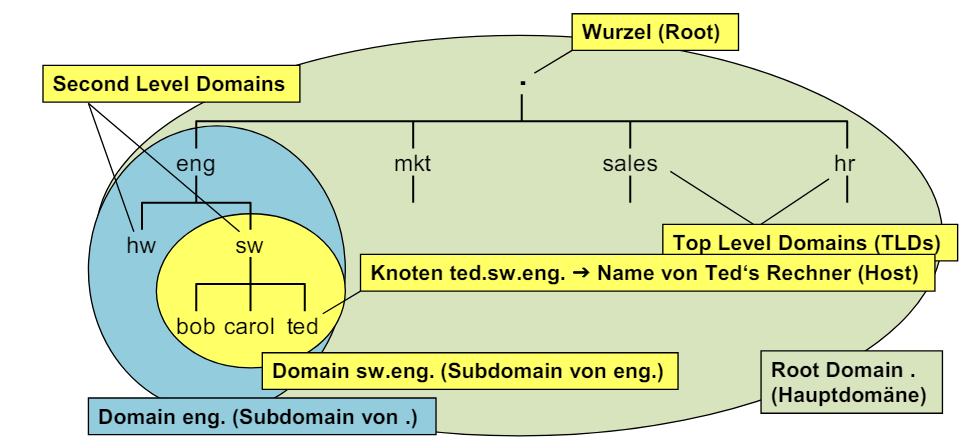
\includegraphics[width=0.8\linewidth]{images/dns_explained.png}
\end{definition}

\begin{concept}{Verwaltung von Domains} NS = Name Server
    \begin{itemize}
        \item DNS wird verteilt betrieben (verteilt, nicht repliziert)
        \item NS: für 1 Zone (separat administrierter Subtree) verantwortlich
        \begin{itemize}
            \item NS kennt IP-Adressen zu Hostnamen in seiner Zone, NS seiner Subdomänen und Root/TLD NS
        \end{itemize}
        \item min. zwei NS pro Zone: Primary (Master) / Secondary (Slave) 
        \item NS kann eine Unterzone seiner Zone weiter delegieren
    \end{itemize}
\end{concept}

\begin{definition}{DNS Record Types}
    \begin{itemize}
        \item A: IPv4 Adresse des gesuchten Hosts (32 Bit)
        \item AAAA: IPv6 Adresse des gesuchten Hosts (128 Bit)
        \item MX: Mail Exchange Record, Mail Server für die Domain 
        \item NS: Name Server Record, Name Server Name für eine Zone
        \item CNAME: Canonical Name (primärer Name), für Alias zum Host
        \item TXT: Text Record, für beliebige Informationen
    \end{itemize}
\end{definition}

\begin{definition}{Reverse DNS Lookup}\\
    Authentisierung: Ein Server identifiziert/authentifiziert einen Client anhand des Namens, nicht anhand der IP-Adresse
\end{definition}

\begin{example2}{DNS-Abfragen auswerten} DNS verwendet Port 53 (UDP)
    \begin{itemize}
        \item Resolver: lokale Software, kommuniziert mit Name Server 
    \end{itemize}
    Beispiel: Anwendung benötigt die IP-Adresse von bob.sw.eng.\\
    \resizebox{\linewidth}{!}{
    FQDN = bob.sw.eng., Root = ., TLD = eng, Second Level Domain = sw}

        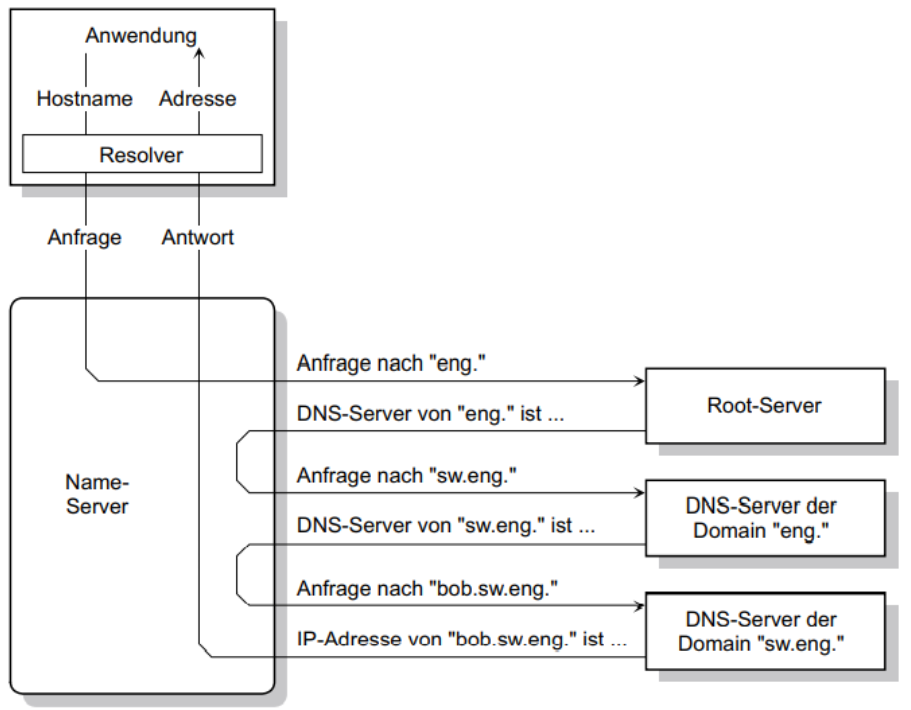
\includegraphics[width=0.9\linewidth]{images/example_dns.png}        
\end{example2}

\columnbreak



\subsubsection{DHCP - Dynamic Host Configuration Protocol}

\begin{definition}{Bezug IP-Adresse} Lokal konfiguriert (static IP)\\
    Bezug der IP-Adresse über das Netzwerk mit DHCP
        \begin{itemize}
            \item erlaubt dynamische Zuteilung aus dem lokalen Adressbereich
        \end{itemize}
\end{definition}

\begin{concept}{Dynamische Zuweisung von IP-Adressen}
    \begin{itemize}
        \item Client verlangt eine IP-Adresse (DHCP Request)
        \item DHCP-Server erteilt eine freie Adresse für definierte Lease Time, oft 10 Minuten (DHCP-Response)
        \item Vor Ablauf der Lease Time: Client erneuert Lease
        \item Client, der Netz verlässt, erneuert Lease nicht: Adresse wieder frei
    \end{itemize}
\end{concept}



\begin{KR}{Ablauf DHCP} Reserviert nur IP’s von aktiven Geräten
    \begin{enumerate}
        \item Client sucht DHCP Server mittels Broadcast
        \item DHCP Server antwortet (DHCP offer)
        \item Der Client wählt einen Server und fordert eine Auswahl der angebotenen Parameter (DHCP request)
        \item Der Server bestätigt mit einer Message, welche die endgültigen Parameter enthält
        \item Vor Ablauf der Lease-Time erneuert der Client die Adresse.
    \end{enumerate}
\end{KR}

\begin{definition}{DHCP Paketformat}\\
    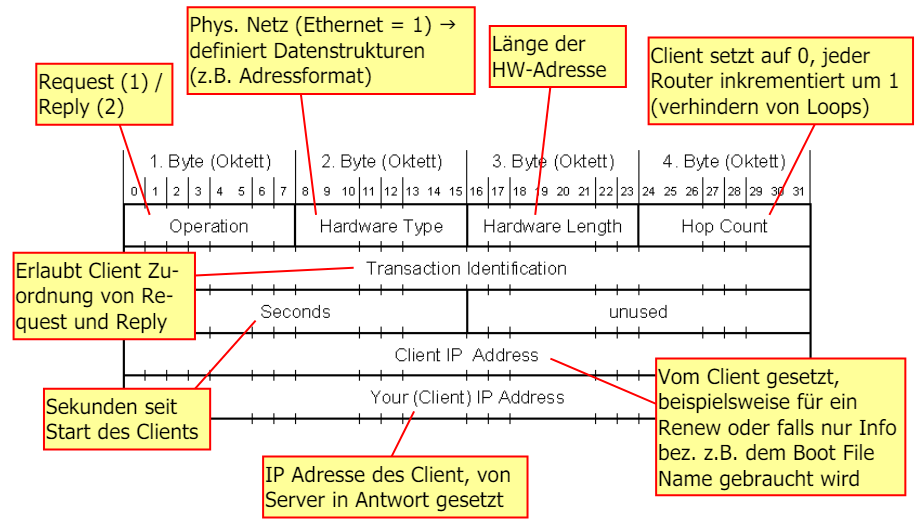
\includegraphics[width=1\linewidth]{images/dhcp_format1.png}

    \vspace{2mm}

    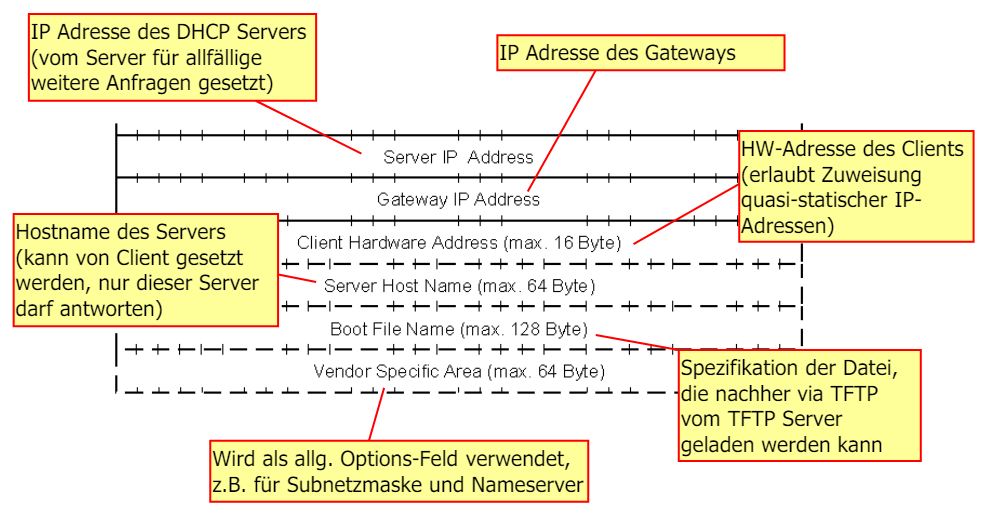
\includegraphics[width=1\linewidth]{images/dhcp_format2.png}
\end{definition}

\subsubsection*{Von A bis Z: Aufruf einer Webseite}

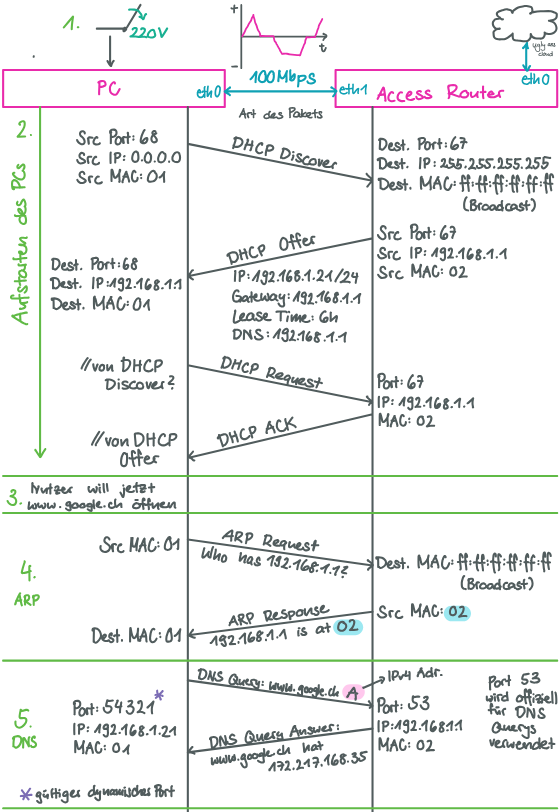
\includegraphics[width=1\linewidth]{images/atoz1.png}\\
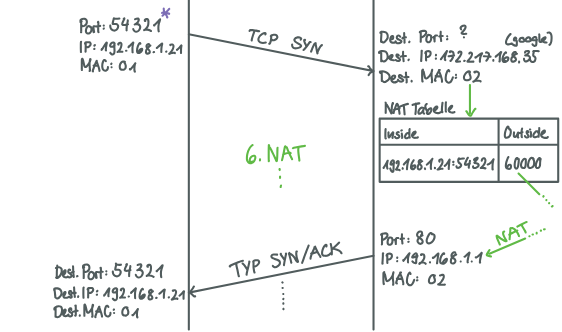
\includegraphics[width=1\linewidth]{images/atoz2.png}



\begin{example2}{Ports{,} Adressen und Routingtabellen} für A-Z Beispiel!\\
    \textcolor{pink}{PC:} UDP-Port = 67, IP = ?, MAC = 01:01:01:01:01:01\\
    Routingtabelle:\\
    \begin{tabular}{|c|c|c|}
        \hline
        Netzadresse + Maske & Port & Gateway\\
        \hline
        192.168.1.0/24 & eth0 & direkt\\
        \hline
        default & eth0 & 192.168.1.1\\
        \hline
    \end{tabular}

    \vspace{2mm}

    \textcolor{pink}{Access Router:} DNS Port = 53, UDP-Port = 67
    \begin{itemize}
        \item Interne IP = 192.168.1.1
        \item Externe IP = 195.1.2.1
        \item MAC = 00:02:02:02:02:02
    \end{itemize}
    Routingtabelle:\\
    \begin{tabular}{|c|c|c|}
        \hline
        Netzadresse + Maske & Port & Gateway\\
        \hline
        192.168.1.0/24 & eth1 & direkt\\
        \hline
        default & eth0 & 195.1.2.1\\
        \hline
    \end{tabular}

\end{example2}
\subsubsection{NAT - Network Address Translation}

\begin{definition}{NAT (Port Mapping)} Port-basierte NAT (NAPT) {\tiny (Boomer Paranoia)}    
    \begin{itemize}
        \item Ersetzt private IP-Adr. durch public IP des Gateways/Routers
        \item Ersetzt private Port-Nr. des Hosts durch freie zulässige Port-Nr. des Gateways/Routers
        \item Mapping privater IP-Adr. und Port-Nr. zur öffentlichen Port-Nr.
                \\auch statisch möglich, aber nur Port-Nr wird übernommen
    \end{itemize}
    Problem mit NAT: Verletzung des OSI-Layer-Konzepts\\
    Um Port im TCP Header zu ändern müssen Daten im IP-Frame verändert werden 
    $\rightarrow$ Netzwerk-Funktion greift auf den Transport Header zu,
    IP-Adresse/Portnummer werden dabei verändert\\
        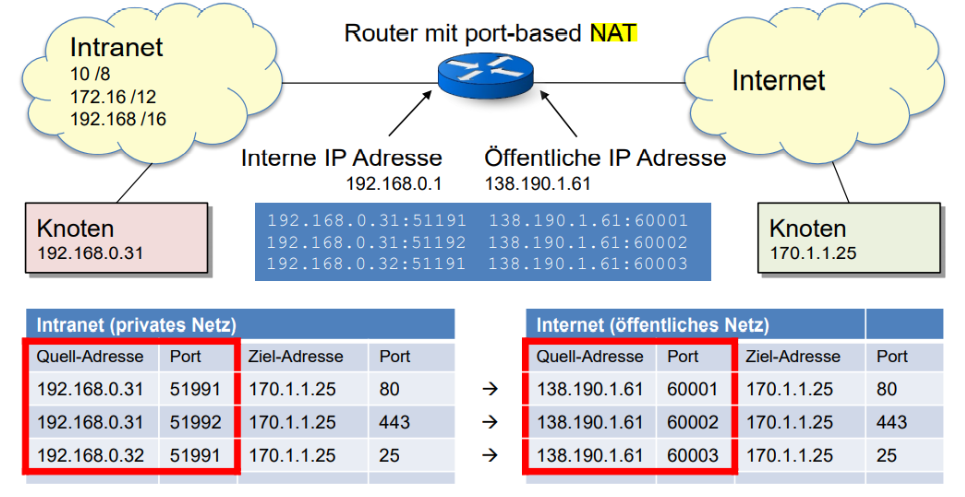
\includegraphics[width=1\linewidth]{images/NAT.png}
\end{definition}
\begin{remark}
    $\forall$ Hosts im privaten Netz 192.168.0.0/8: Default-Gateway 192.168.0.1
\end{remark}

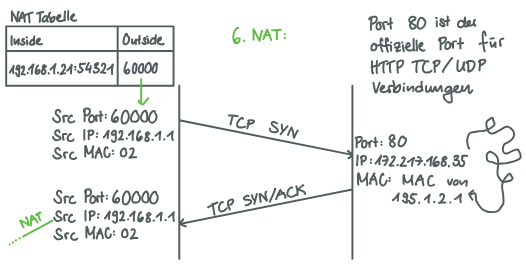
\includegraphics[width=1\linewidth]{images/atoz3.png}



